\documentclass{standalone}
\usepackage{tikz}
\usepackage{ctex,siunitx,ninecolors}
\setCJKmainfont{Noto Serif CJK SC}
\usepackage{tkz-euclide}
\usepackage{amsmath}
\usetikzlibrary{patterns, calc}
\usetikzlibrary {decorations.pathmorphing, decorations.pathreplacing, decorations.shapes,}
\begin{document}
\small
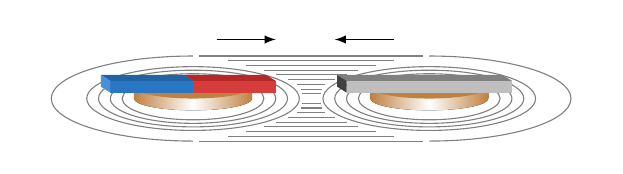
\begin{tikzpicture}[>=latex,scale=1.5]
  \useasboundingbox(-2.4,-0.4)rectangle(2.4,0.6);
  \foreach \x in {-1,1}
  {
    \draw[gray](\x,0)ellipse(0.6 and 0.18);
    \draw[gray](\x,0)ellipse(0.7 and 0.21);
    \draw[gray](\x,0)ellipse(0.8 and 0.24);
    \draw[gray](\x,0)ellipse(0.9 and 0.27);
    \fill[left color=brown,right color=brown,middle color=white](\x,0)ellipse(0.5 and 0.1);
    \fill[left color=brown,right color=brown,middle color=white](\x-0.5,0)rectangle(\x+0.5,0.1);
    \fill[brown](\x,0.1)ellipse(0.5 and 0.1);
  }
  \draw[gray](-1,0.36)arc(90:270:1.2 and 0.36);
  \draw[gray](1,0.36)arc(90:-90:1.2 and 0.36);
  \draw[gray](-0.95,0.36)--(0.95,0.36)(-0.95,-0.36)--(0.95,-0.36);
  \foreach \x/\y in {0.7/0.32,0.55/0.28,0.4/0.24,0.3/0.20,0.2/0.16,0.12/0.12,0.09/0.08,0.08/0.04}
  {
    \draw[gray](\x,\y)--(-\x,\y);
    \draw[gray](\x,-\y)--(-\x,-\y);
  }

  \fill[lightgray](0.3,0.05)rectangle(1.7,0.15);
  \fill[gray](0.3,0.15)--++(-0.08,0.05)--++(1.4,0)--++(0.08,-0.05)--cycle;
  \fill[darkgray](0.3,0.15)--++(-0.08,0.05)--++(0,-0.1)--++(0.08,-0.05)--cycle;
  \fill[red5](-0.3,0.05)rectangle(-1,0.15);
  \fill[red4](-0.3,0.15)--++(-0.08,0.05)--++(-0.7,0)--++(0.08,-0.05)--cycle;
  \fill[azure5](-1,0.05)rectangle(-1.7,0.15);
  \fill[azure4](-1,0.15)--++(-0.08,0.05)--++(-0.7,0)--++(0.08,-0.05)--cycle;
  \fill[azure6](-1.7,0.15)--++(-0.08,0.05)--++(0,-0.1)--++(0.08,-0.05)--cycle;
  \draw[->] (-0.8,0.5)--++(0.5,0);
  \draw[->](0.7,0.5)--++(-0.5,0);
  % \fill[darkgray](0.3,0.15)--++(-0.08,0.05)--++(0,-0.1)--++(0.08,-0.05)--cycle;
  \end{tikzpicture}
\end{document}